\documentclass{standalone}
\usepackage{amsmath, graphicx, siunitx}
\usepackage{tikz}
\usetikzlibrary{arrows, calc, backgrounds, positioning}

\newcommand\dataline[5]{
    \draw [line width=#1 mm, color=gray] (#3) to [#5] (#4);
    \draw [line width=#2 mm, color=blue] (#3) to [#5] (#4);
}

\tikzstyle{background} = [fill=green!5!white,draw=green!75!black,very thick]
\tikzstyle{titlebox} = [fill=green!75!black,text=black,rounded corners]

\tikzstyle{disk}       = [rectangle,fill=black!20,align=left,rotate=90,inner sep=0]
\tikzstyle{controller} = [rectangle,fill=red!20,align=left,inner sep=0]
\tikzstyle{network}    = [rectangle,fill=blue!20,align=left,inner sep=0]
\tikzstyle{switch}     = [rectangle,fill=green!20,align=left,inner sep=0]

% Network latency is 0.004 ms
%  Disk   latency is 4     ms

% If the sep between NIC and switch is 2cm, then using a log scale, the
% disks are (2 cm) * log(4 / 0.004) = 13.8 cm below the RAID controller

\begin{document}
    \begin{tikzpicture}
        \node[controller]           (raid)                                        {RAID controller:\\ 63 Gb/s interface,\\ forwards 40 Gb/s};
        \node[disk,anchor=north]    (disk 1)     at ($(raid.south)+(-1in, -3cm)$) {\begin{minipage}{2.7cm}
                                                                                       SSD 1:\\
                                                                                       12 Gb/s interface,\\
                                                                                       sends 4 Gb/s,\\
                                                                                       \SI{4}{\milli\second} latency
                                                                                   \end{minipage}
                                                                                   \begin{minipage}{1cm}
                                                                                       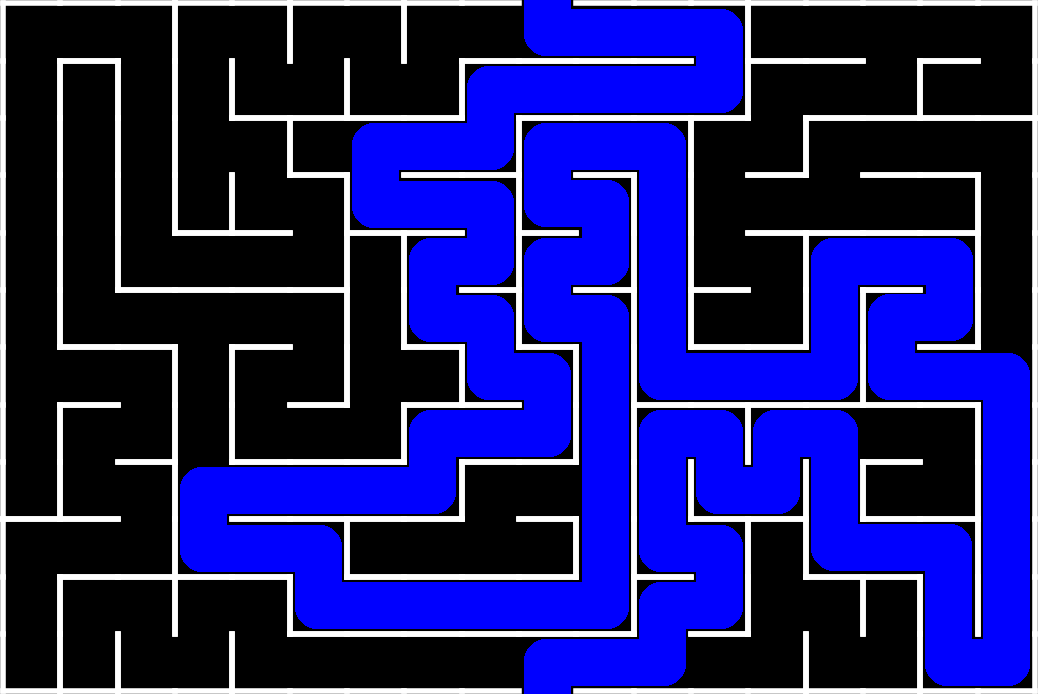
\includegraphics[height=\textwidth,angle=90,origin=c]{maze-tortuous}
                                                                                   \end{minipage}};
        \node[disk]                 (disk 2)     at ($(disk 1) + (2cm, 0)$)       {\begin{minipage}{2.7cm}
                                                                                       SSD 2:\\
                                                                                       12 Gb/s interface,\\
                                                                                       sends 4 Gb/s,\\
                                                                                       \SI{4}{\milli\second} latency
                                                                                   \end{minipage}
                                                                                   \begin{minipage}{1cm}
                                                                                       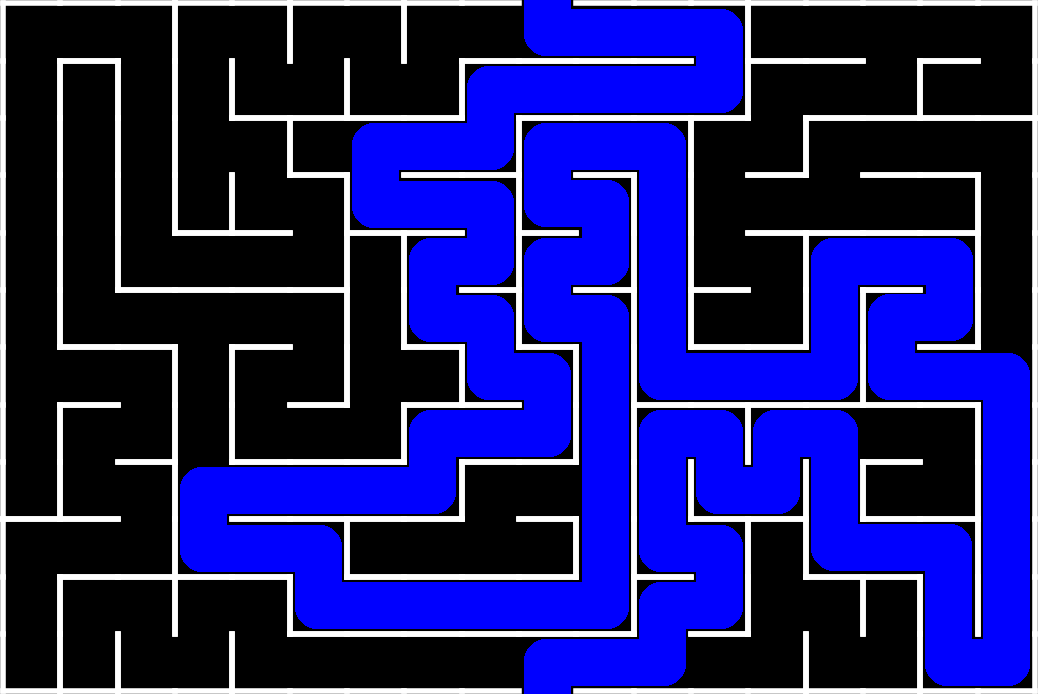
\includegraphics[height=\textwidth,angle=270,origin=c]{maze-tortuous}
                                                                                   \end{minipage}};
        \node                       (dots)       at ($(disk 2) + (1.5cm, 0)$)     {$\cdots$};
        \node[disk]                 (disk N)     at ($(dots) + (+1.5cm, 0)$)      {\begin{minipage}{2.7cm}
                                                                                       SSD $N$:\\
                                                                                       12 Gb/s interface,\\
                                                                                       sends 4 Gb/s,\\
                                                                                       \SI{4}{\milli\second} latency
                                                                                   \end{minipage}
                                                                                   \begin{minipage}{1cm}
                                                                                       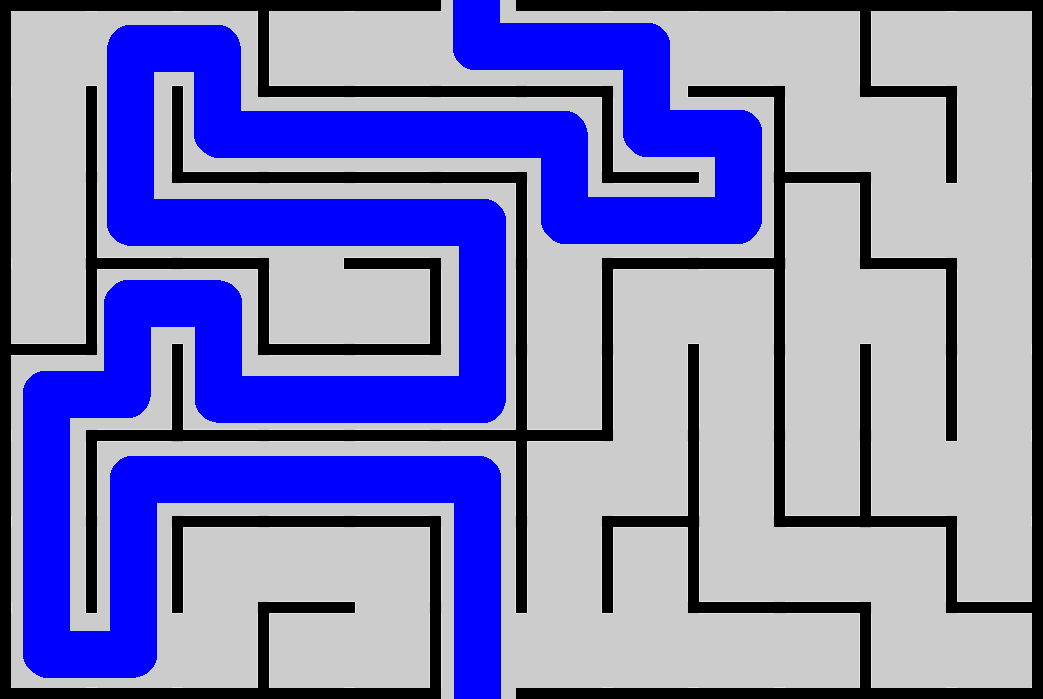
\includegraphics[height=\textwidth,angle=90,origin=c]{maze-tortuous-mirror}
                                                                                   \end{minipage}};
        \node[network]              (nic)        [right=of raid]                  {\begin{minipage}{2.7cm}
                                                                                       network card:\\
                                                                                       56 Gb/s interface,\\
                                                                                       forwards 40 Gb/s
                                                                                   \end{minipage}
                                                                                   \begin{minipage}{1cm}
                                                                                       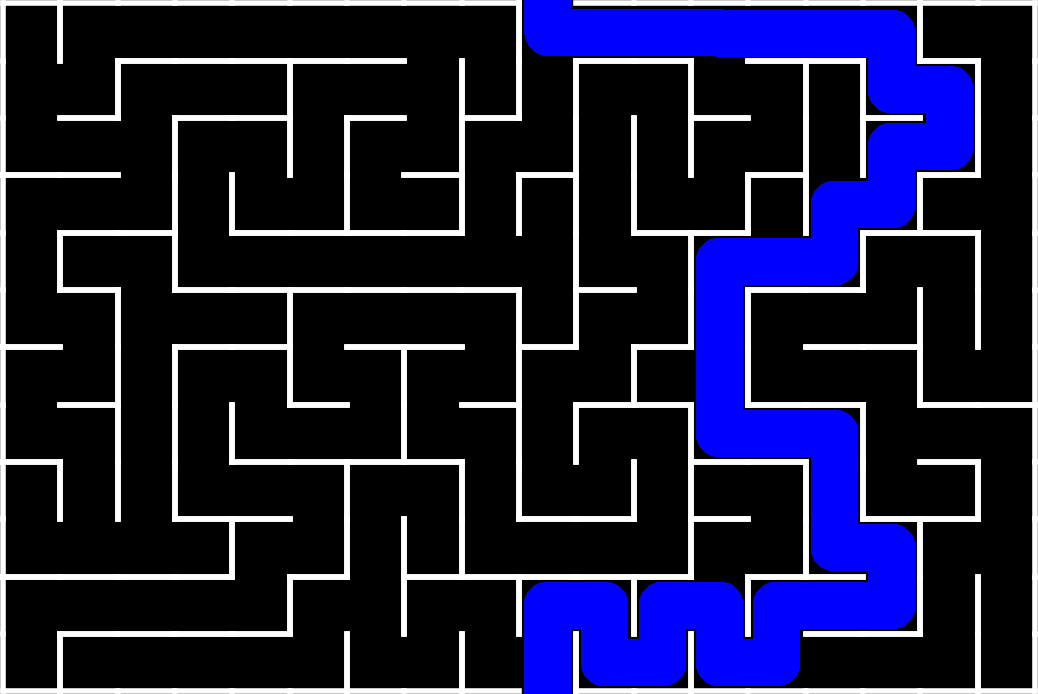
\includegraphics[height=\textwidth,angle=90,origin=c]{maze-direct}
                                                                                   \end{minipage}};
        \node[switch,anchor=west]   (switch)     [right=of nic]                   {network switch:\\
                                                                                   56 Gb/s interfaces,\\
                                                                                   forwards 40 Gb/s,\\
                                                                                   \SI{0.004}{\milli\second} latency};
        \node[network,anchor=south] (node 1 nic) [above=of switch]                {node 1 network card:\\
                                                                                   56 Gb/s interface,\\
                                                                                   receives 20 Gb/s};
        \node[network,anchor=north] (node 2 nic) [below=of switch]                {node 2 network card:\\
                                                                                   56 Gb/s interface,\\
                                                                                   receives 20 Gb/s};

        \node[titlebox] (server) at ($(raid.north)+(2cm, 0.5cm)$) {\textbf{Server}};

        \dataline{1.2}{0.4}{disk 1.east}{raid}{out=90,in=260};
        \dataline{1.2}{0.4}{disk 2.east}{raid}{out=90,in=270}
        \dataline{1.2}{0.4}{disk N.east}{raid}{out=90,in=280}
        \dataline{5.6}{4.0}{raid}{nic}{}
        \dataline{5.6}{4.0}{nic}{switch}{}
        \dataline{4.0}{2.0}{switch}{node 1 nic}{}
        \dataline{4.0}{2.0}{switch}{node 2 nic}{}

        \begin{pgfonlayer}{background}
		    \draw [background] ($(nic.north east)+(0, 0.35cm)$) rectangle ($(disk 1.north west)$);
        \end{pgfonlayer}
    \end{tikzpicture}
\end{document}
